\documentclass[solution, letterpaper]{cs121}

\usepackage{tikz-qtree}
\usepackage{graphicx}
\usepackage{color}
\usepackage{amsfonts}
\usepackage{amsmath}
\usepackage[english]{babel}
\usepackage[utf8]{inputenc}
\usepackage{ae,aecompl}

% allow metapost figures to be included inline
% note: you must invoke latex using:
%
%     pdflatex -shell-escape <inputfile>
%
% to allow it to invoke external commands. See the very end of the
% document as well.
\usepackage{emp,ifpdf}
\usepackage{graphicx}

% convert metapost figures to .eps or .pdf automatically when
% including them
\ifpdf\DeclareGraphicsRule{*}{mps}{*}{}\fi

% include the metapost macros
\empprelude{input boxes; input theory}

%% Please fill in your name and collaboration statement here.
%\newcommand{\studentName}{Renzo Lucioni and Daniel Broudy}
%\newcommand{\collaborationStatement}{I collaborated with...}
\newcommand{\solncolor}{red}
\begin{document}

% create a metapost file for figures to be dumped to.  It's easiest
% to use a single file for all the figures in the document
\begin{empfile}

\header{4}{April 12, 2013, at 12:00 PM}{}{}

%%%%%%%%%%%%%%%%%%%%%%%%%%%%%%%%%%%%%%%%%%%%%%%%%%%%
\problem{14} %1

\subproblem %a
The diagram below illustrates the directed graph structure of the network.

\begin{center}
\begin{emp}(0,0)
  % it's good practice to pick a basic size unit and make all your
  % distances relative to that unit
  u := 2cm;
  ubernodes;
  % create a node, and position its center at the origin
  node.q1(btex $MAI$ etex); q1.c = origin;

  % position the other nodes relative to it
  node.q2(btex $NAI$ etex); q2.c = q1.c + (1.5u,0);
  node.q3(btex $RD$ etex); q3.c = q1.c + (3u,0);
  node.q4(btex $VRAS$ etex); q4.c = q1.c + (0.75u,-1.5u);
  node.q5(btex $SMOS$ etex); q5.c = q1.c + (2.25u,-1.5u);
  node.q6(btex $VP$ etex); q6.c = q1.c + (1.5u,-3u);

  % mark q1 as a start node
  %makestart(q1);

  % mark q4 as an accept node
  %makefinal(q1);

  % draw the nodes
  drawboxed(q1,q2,q3,q4,q5,q6);

  edge(q1,q4,right,btex etex);
  edge(q2,q4,right,btex etex);
  edge(q3,q5,right,btex etex);
  edge(q4,q6,right,btex etex);
  edge(q5,q6,right,btex etex);

\end{emp}
\end{center}

The following describes a parameterization of the noise in the causal effects of the above dependencies. To begin with, we have the following factorization of the directed graph:
\begin{equation*}
\resizebox{1\hsize}{!}{$P(RD,SMOS,VRAS,MAI,NAI,VP) = P(MAI)P(NAI)P(RD)P(VRAS | MAI, NAI)P(SMOS | RD)P(VP | VRAS, SMOS)$}
\end{equation*}

$MAI$, $NAI$, and $RD$ are root nodes (i.e., nodes with no predecessors). As such, they are not conditional on any other attributes. Thus, we have the following three prior probability tables.
\begin{center}
\begin{tabular}{ c |c }
   $MAI = 0$ & $MAI = 1$ \\
   \hline
  0.6 & 0.4 \\
\end{tabular}
\end{center}

\begin{center}
\begin{tabular}{ c |c }
   $NAI = 0$ & $NAI = 1$ \\
   \hline
  0.3 & 0.7 \\
\end{tabular}
\end{center}

\begin{center}
\begin{tabular}{ c |c }
   $RD = 0$ & $RD = 1$ \\
   \hline
  0.2 & 0.8 \\
\end{tabular}
\end{center}

The remaining nodes, $VRAS$, $SMOS$, and $VP$, are non-root nodes. Therefore, each is associated with a conditional probability table. $VRAS$ is conditional on $MAI$ and $NAI$, and is associated with the following conditional probability table.
\begin{center}
\begin{tabular}{ c |c c }
   & $VRAS = 0$ & $VRAS = 1$ \\
   \hline
  $MAI = 0, NAI = 0 $ & 1.0 & 0.0 \\
  $MAI = 0, NAI = 1 $ & 0.5 & 0.5 \\
  $MAI = 1, NAI = 0 $ & 0.4 & 0.6 \\
  $MAI = 1, NAI = 1 $ & 0.2 & 0.8 \\
\end{tabular}
\end{center}

$SMOS$ is conditional on $RD$, and is associated with the following conditional probability table.
\begin{center}
\begin{tabular}{ c |c c }
   & $SMOS = 0$ & $SMOS = 1$ \\
   \hline
  $RD = 0$ & 0.8 & 0.2 \\
  $RD = 1$ & 0.5 & 0.5 \\
\end{tabular}
\end{center}

$VP$ is conditional on $VRAS$ and $SMOS$, and is associated with the following conditional probability table.
\begin{center}
\begin{tabular}{ c |c c }
   & $VP = 0$ & $VP = 1$ \\
   \hline
  $VRAS = 0, SMOS = 0 $ & 0.98 & 0.02 \\
  $VRAS = 0, SMOS = 1 $ & 0.3 & 0.7 \\
  $VRAS = 1, SMOS = 0 $ & 0.45 & 0.55 \\
  $VRAS = 1, SMOS = 1 $ & 0.001 & 0.999 \\
\end{tabular}
\end{center}

\subproblem %b
We made the assumption that $VRAS$ and $SMOS$ are independent. This assumption is expressed in the graph structure above. We made this decision because silly messages on the screen do not necessarily have any bearing on whether your antivirus software reports that a virus is present on your computer, and vice-versa. That is, $SMOS$ and $VRAS$ are not necessarily related. It would be plausible for us to \emph{not} make this assumption, meaning we would have added an edge from $SMOS$ to $VRAS$ to our network. Including this new edge would be reasonable because if you have silly messages on your screen, you might also expect your antivirus to report that there is a virus present on your computer, whether or not one is actually present notwithstanding.

\subproblem %c
The diagram below illustrates the directed graph structure of the network with the new variables $VRM$ and $VRN$ included.

\begin{center}
\begin{emp}(0,0)
  % it's good practice to pick a basic size unit and make all your
  % distances relative to that unit
  u := 2cm;
  ubernodes;
  % create a node, and position its center at the origin
  node.q1(btex $MAI$ etex); q1.c = origin;

  % position the other nodes relative to it
  node.q2(btex $NAI$ etex); q2.c = q1.c + (1.5u,0);
  node.q3(btex $RD$ etex); q3.c = q1.c + (3u,0);
  node.q4(btex $VRAS$ etex); q4.c = q1.c + (0.75u,-2.5u);
  node.q5(btex $SMOS$ etex); q5.c = q1.c + (2.25u,-2.5u);
  node.q6(btex $VP$ etex); q6.c = q1.c + (1.5u,-4u);
  node.q7(btex $VRM$ etex); q7.c = q1.c + (.3u,-1.2u);
  node.q8(btex $VRN$ etex); q8.c = q1.c + (1.2u,-1.2u);

  % mark q1 as a start node
  %makestart(q1);

  % mark q4 as an accept node
  %makefinal(q1);

  % draw the nodes
  drawboxed(q1,q2,q3,q4,q5,q6,q7,q8)

  edge(q7,q4,right,btex etex);
  edge(q8,q4,right,btex etex);
  edge(q3,q5,right,btex etex);
  edge(q4,q6,right,btex etex);
  edge(q5,q6,right,btex etex);
  edge(q1,q7,right,btex etex);
  edge(q2,q8,right,btex etex);

\end{emp}
\end{center}

$VRM$ is conditional on $MAI$, and is associated with the following conditional probability table.
\begin{center}
\begin{tabular}{ c |c c }
   & $VRM = 0$ & $VRM = 1$ \\
   \hline
  $MAI = 0$ & 1.0 & 0.0 \\
  $MAI = 1$ & 0.4 & 0.6 \\
\end{tabular}
\end{center}

$VRN$ is conditional on $NAI$, and is associated with the following conditional probability table.
\begin{center}
\begin{tabular}{ c |c c }
   & $VRN = 0$ & $VRN = 1$ \\
   \hline
  $NAI = 0$ & 1.0 & 0.0 \\
  $NAI = 1$ & 0.5 & 0.5 \\
\end{tabular}
\end{center}

$VRAS$ is now conditional on $VRM$ and $VRN$, and is associated with the following conditional probability table.
\begin{center}
\begin{tabular}{ c |c c }
   & $VRAS = 0$ & $VRAS = 1$ \\
   \hline
  $VRM = 0, VRN = 0 $ & 1.0 & 0.0 \\
  $VRM = 0, VRN = 1 $ & 0.0 & 1.0 \\
  $VRM = 1, VRN = 0 $ & 0.0 & 1.0 \\
  $VRM = 1, VRN = 1 $ & 0.0 & 1.0 \\
\end{tabular}
\end{center}

\subproblem %d
Including nodes $VRM$ and $VRN$ helps the modeling process by making the inference more accurate? 

%%%%%%%%%%%%%%%%%%%%%%%%%%%%%%%%%%%%%%%%%%%%%%%%%%%%
\problem{24} %2
\subproblem 
- For graph (a) there are no variables that are Independent of A given the knowledge of B. There is a head-tail or a tail-tail connection to all other nodes (or a path that is a D-separation of these) and none of the middle nodes in these tail-tail or head-tail's are known so they do not blocking. Knowledge of B does block the dependence of A on D through B but A is still not independent of D through a different path. Therefore none of the nodes are independent of A given knowledge of B.\\
%see Reading http://research.microsoft.com/en-us/um/people/cmbishop/prml/Bishop-PRML-sample.pdf 
%page 378.

- For graph (b) only F and C are independent of A given J. In this case we would think the path through G would be blocked because G is is a head to head node. With the knowledge of J, G does not block the path between A and D because J is a decedent node of G, this creates an induced dependence between A and D. This is not the case between D and E, H does not create induced dependence because it is unknown and none of its descendants are known, that being said the existence of B, an unknown tail tail connection means there is a dependence between D and E. Now finally between E and F we get independence because I is a head-head node and none of its descendants are known. This leaves us with the conclusion that F and C are the only two nodes that are independent of A when J is known. Knowledge of J induces a lot more dependence in this directed graph.

\subproblem \\%b
%P(A,B,C,D,E,F,G,H,I) = P(G)P(H)P(I|G,H)P(D|G)P(E|G)(P(F|H)P(C|E,F)P(B|D)P(A|B,C)\\
%TODO: make smaller
\begin{equation*}
\resizebox{1\hsize}{!}{$P(A,B,C,D,E,F,G,H,I) = \frac{1}{Z}\Psi_1(G)\Psi_2(H)\Psi_3(I,G,H)\Psi_4(D,G)\Psi_5(E,G)\Psi_6(F,H)\Psi_7(C,E,F)\Psi_8(B,D)\Psi_9(A,B,C)$}
\end{equation*}
%P(A,B,C,D,E,F,G,H,I) = P(A)P(B)P(C)P(D|B)P(E|B)P(F|C)P(G|A,D)P(H|D,E)P(I|E,F)P(J|G)\\
%TODO: make smaller
\begin{equation*}
\resizebox{1\hsize}{!}{$P(A,B,C,D,E,F,G,H,I) = \frac{1}{Z}\Psi_1(A)\Psi_2(B)\Psi_3(C)\Psi_4(D,B)\Psi_5(E,B)\Psi_6(F,C)\Psi_7(G,A,D)\Psi_8(H,D,E)\Psi_9(I,E,F)\Psi_{10}(J,G)$}
\end{equation*}
\subproblem %c
\begin{center}
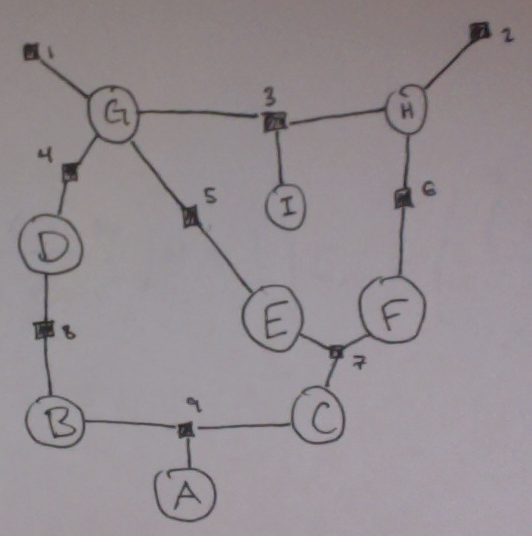
\includegraphics[width=100mm]{factor_graph_a.png}
\end{center}

\begin{center}
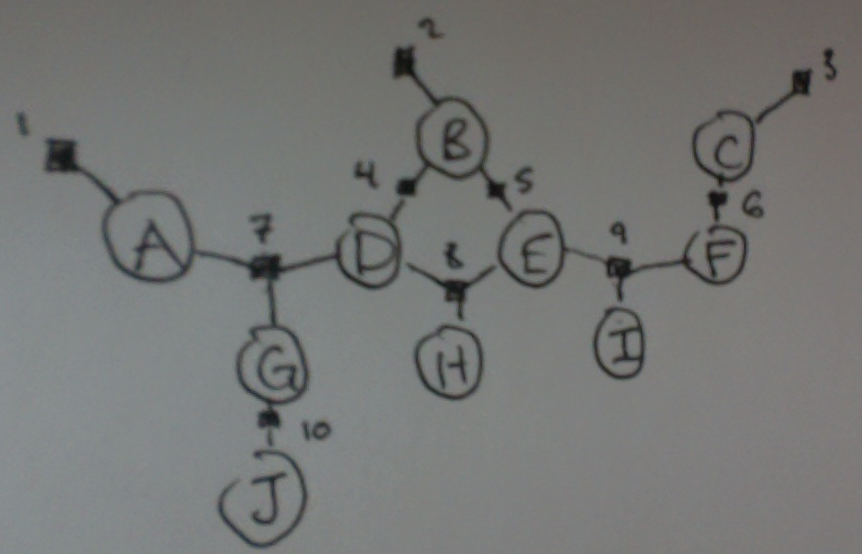
\includegraphics[width=100mm]{factor_graph_b.png}
\end{center}

\subproblem %d

\begin{center}
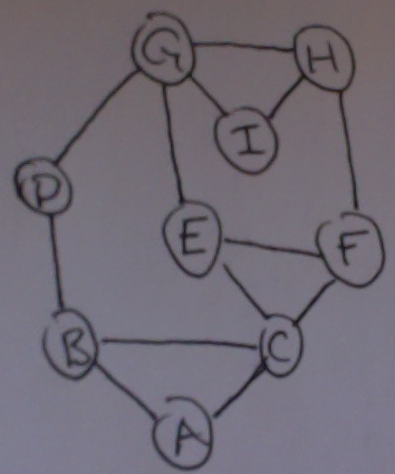
\includegraphics[width=100mm]{undirected_graph_a.png}
\end{center}

\begin{center}
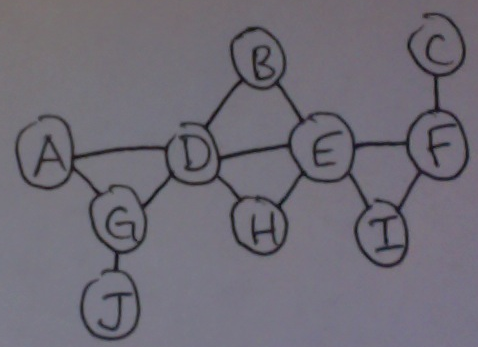
\includegraphics[width=100mm]{undirected_graph_b.png}
\end{center}

%%%%%%%%%%%%%%%%%%%%%%%%%%%%%%%%%%%%%%%%%%%%%%%%%%%%
\problem{25} %3
% Normal(mu, sigma^2)
% (0.2*NormalDistribution[1, 25]) + (0.3*NormalDistribution[-2, 1])+(0.5*NormalDistribution[3, 4])
\subproblem %a
Below is the requested plot of the given density function.
\begin{center}
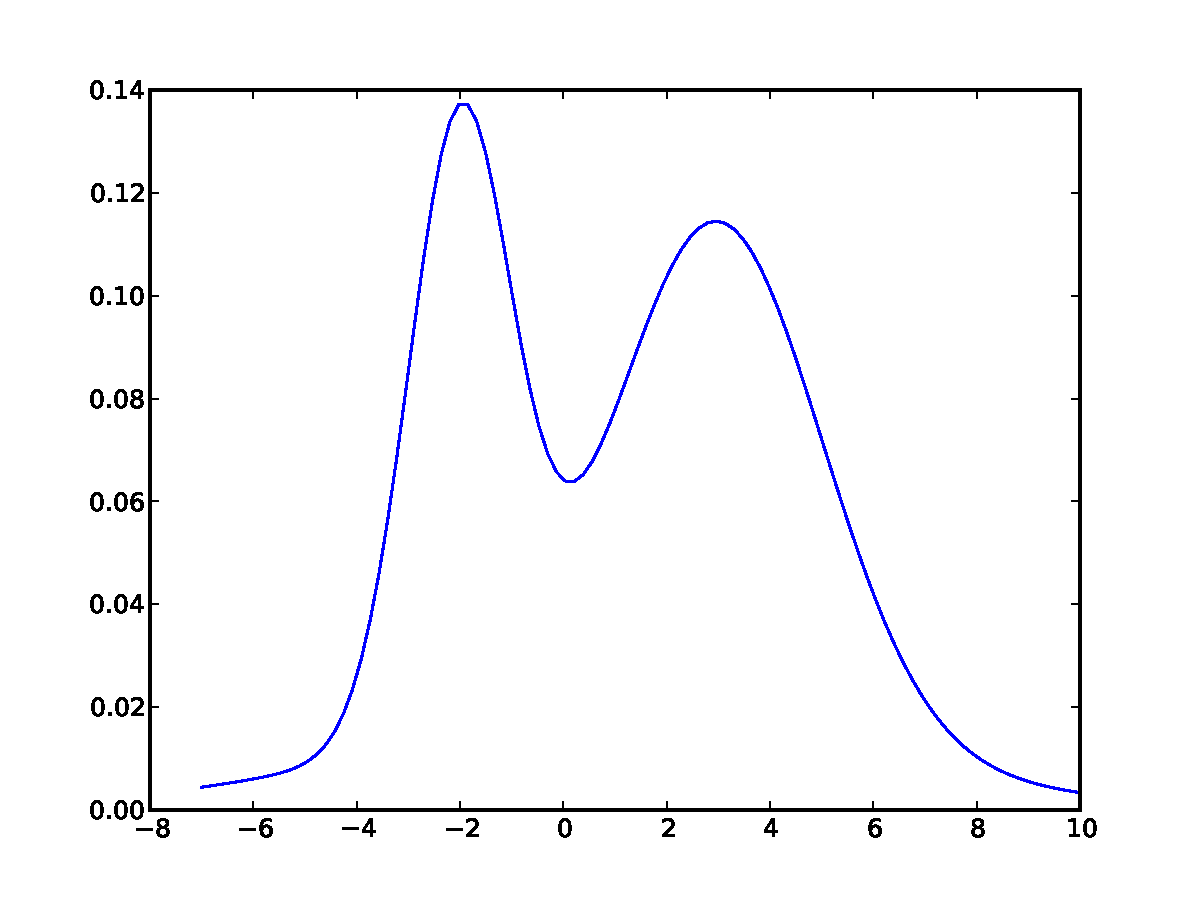
\includegraphics[scale=0.8]{mixture-o-gaussians.pdf}
\end{center}

\subproblem %b
In this problem, we are given three Gaussian densities: $\mathcal{N}(1,25)$, $\mathcal{N}(-2,1)$, and $\mathcal{N}(3,4)$. We are interested in sampling directly from the given mixture of these three Gaussian densities. To generate data directly from the distribution, we use {\tt random.gauss(mu, sigma)}, Python's built-in function for sampling from a Gaussian distribution, and a biased ``three-sided coin." That is, we randomly generate a number between 1 and 10, inclusive. If the number is 1 or 2, we sample from the first Gaussian. If the number is 3, 4, or 5, we sample from the second Gaussian. If the number is 6, 7, 8, 9, or 10, we sample from the third Gaussian distribution. The effect is sampling from the first Gaussian with probability 0.2, from the second Gaussian with probability 0.3, and from the third Gaussian with probability 0.5. Below is a histogram of 500 samples drawn in this way:
\begin{center}
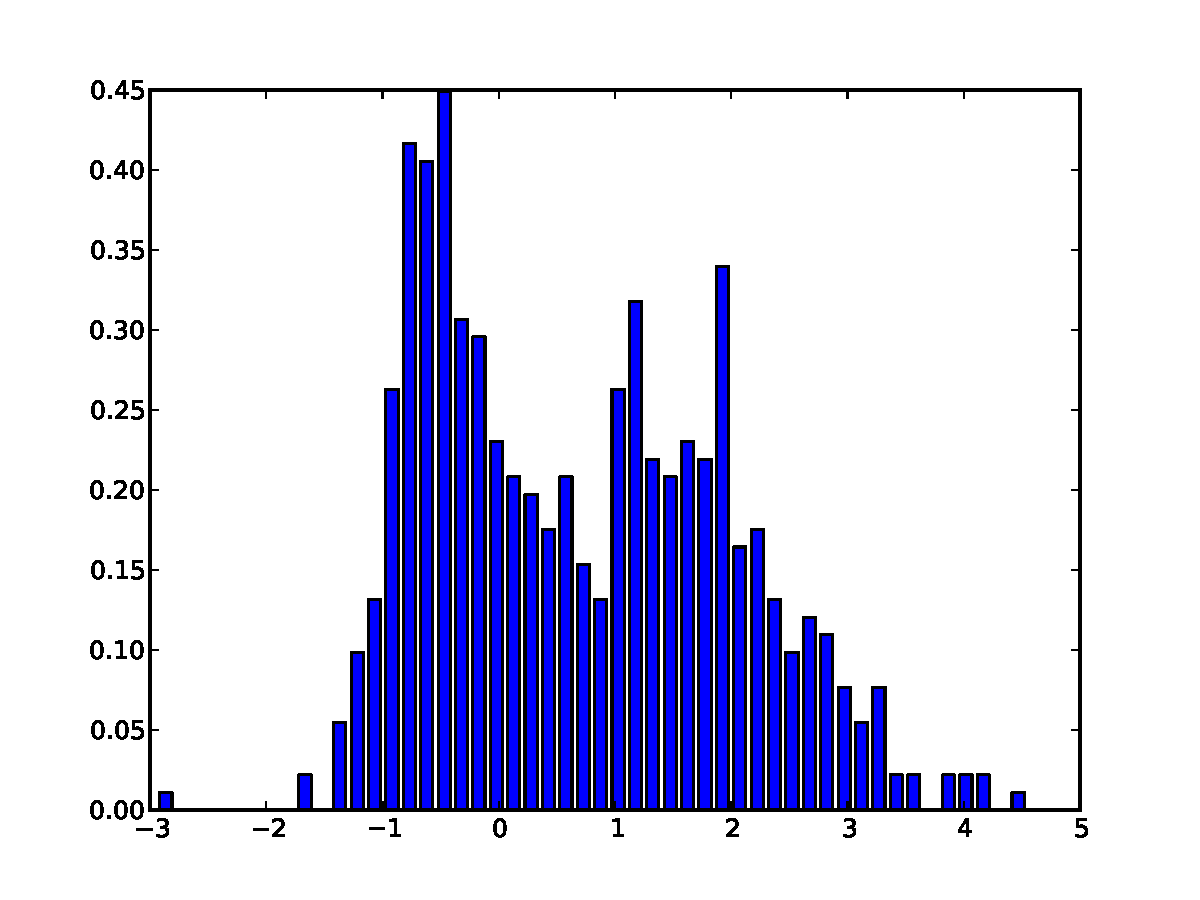
\includegraphics[scale=0.8]{direct-sample-histogram.pdf}
\end{center}

\subproblem %c
In this problem, we pretend we do not know how to perform the ``direct" sampling in (B), and implement a rejection sampler for the given density. We use the upper bounding function $\mathcal{N}(0,24)$ with $c=2$. Below is the requested plot of our upper bounding function against the given density function.
\begin{center}
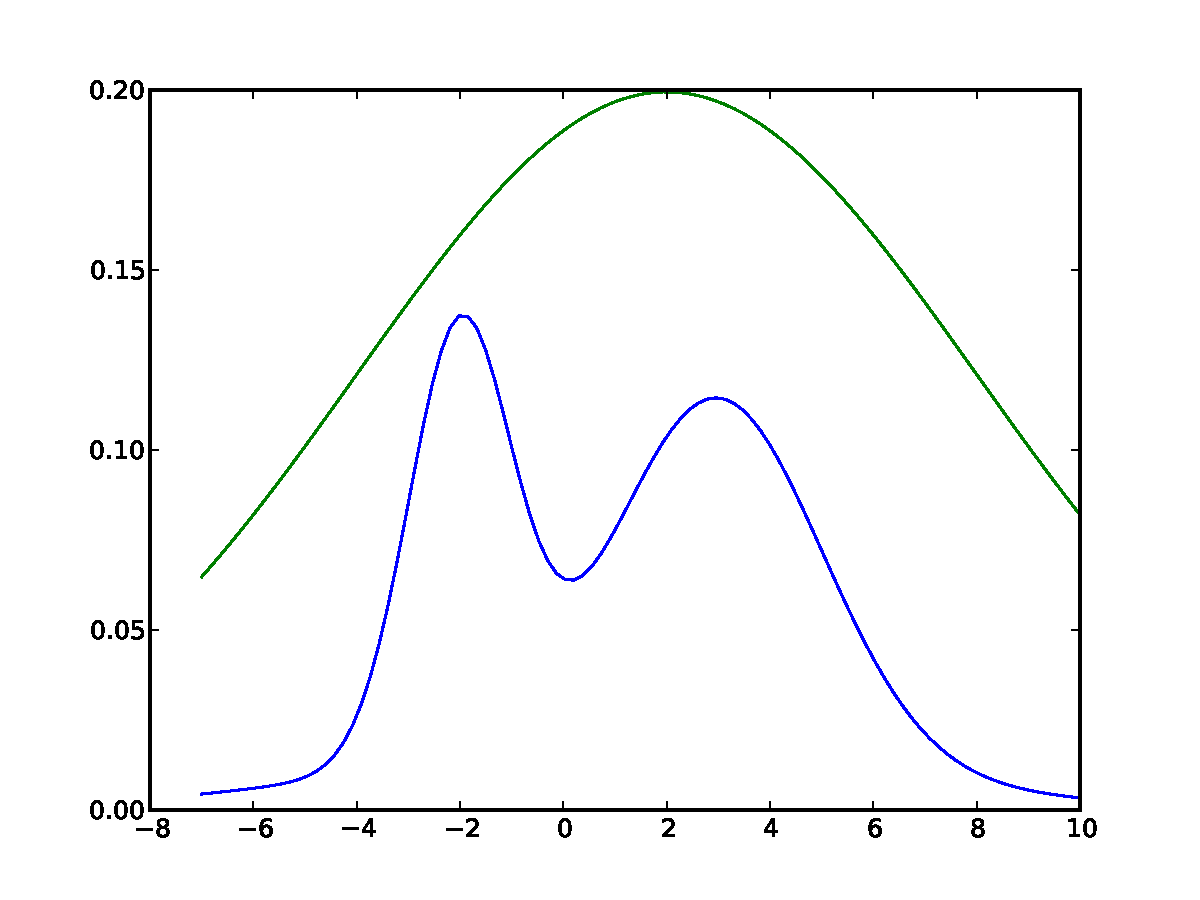
\includegraphics[scale=0.8]{mixture-w-envelope.pdf}
\end{center}

Below is a histogram of 500 samples drawn using our rejection sampler:
\begin{center}
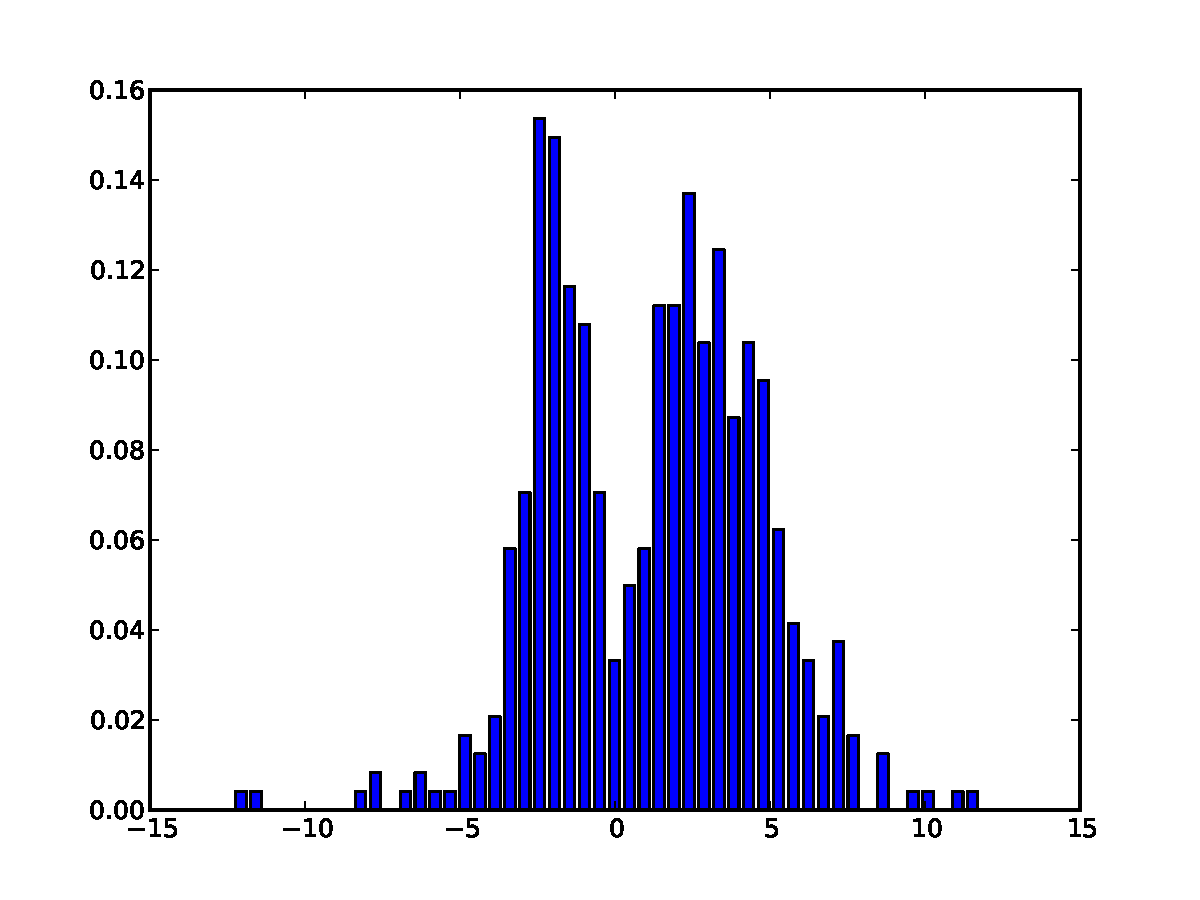
\includegraphics[scale=0.8]{rejection-sample-histogram.pdf}
\end{center}

We got 495 rejections before we got 500 acceptances, constituting a rejection rate of 0.99.

\subproblem %d
In this problem we implement the Metropolis-Hastings algorithm using a simple Gaussian proposal. To begin with, we used a proposal function with a variance of 5. This resulted in an acceptance rate of $0.57$. We then tried using a variance of 15 and found that the histogram became noticeably worse, showing many spikes. The acceptance rate dropped to $0.23$. Next, we tried a small variance of 1. This resulted in a high acceptance rate of $0.87$. The resulting histogram was much smoother than the one with a variance of 15, but was so smooth that it failed to capture the peaks and troughs of the mixture distribution. Finally, we tried a variance of 3, resulting in an acceptance rate of $0.70$, and a relatively smooth histogram which captured the peaks and troughs of the mixture distribution. This histogram is included below. We also experimented with using a burn-in period of 500 samples, but realized that since we already know what our target distribution looks like, the burn-in period is not useful. 

\begin{center}
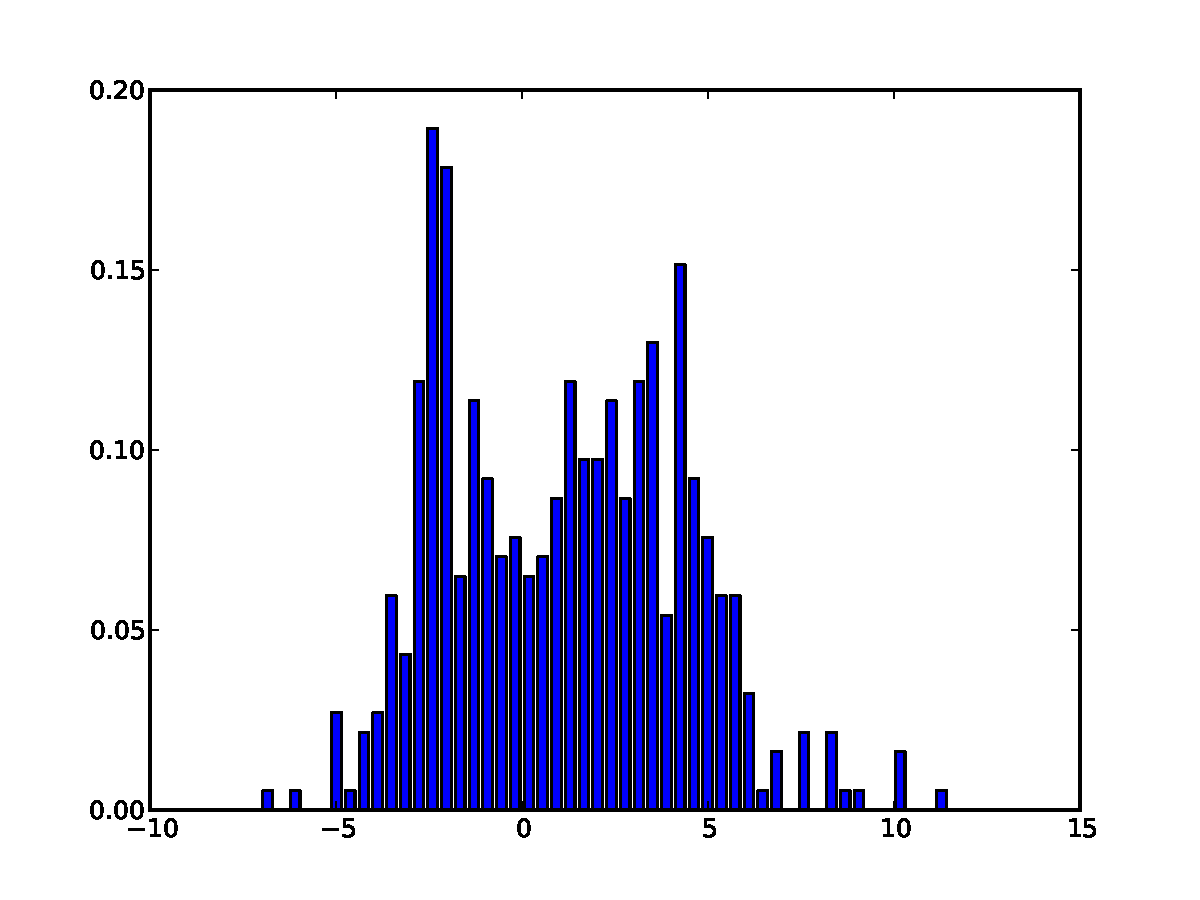
\includegraphics[scale=0.8]{hasty_metro_histogram.pdf}
\end{center}


\end{empfile}

% this invokes metapost on the figures. You must run latex a second
% time for the figures to be included.
\immediate\write18{mpost -tex=latex \jobname}

\end{document}






